\chapter{Metodología de la gestión del proyecto}
\label{chap:metodología}

\drop{A} causa de la multitud de objetivos que se deben realizar para llevar a cabo este \ac{TFG}, es necesario seguir una metodología de trabajo para poder ir desarrollando el proyecto de una forma clara, organizada y acotada en función del tiempo.

Si nos basamos en la definición del \ac{PMI}\footnote{PMI es la asociación profesional sin fines de lucro más importante y de mayor crecimiento a nivel mundial que tiene como misión convertir la gerencia de proyectos como la actividad indispensable para obtener resultados en cualquier actividad de negocios.}, la gestión de proyectos sería la aplicación de herramientas, conocimientos, habilidades, y técnicas para conseguir los objetivos del proyecto. A continuación se van a enumerar las metodologías de gestión más utilizadas, según la referencia \cite{MetodologiasGestion}:  

\begin{enumerate}
\item \acx{PMBOK} \cite{PMBOK}. El \ac{PMI} elaboró este libro, donde se establece todo un conjunto de herramientas y buenas prácticas que todo jefe de proyecto debe conocer y aplicar. El \ac{PMBOK} está orientado a una gestión predictiva de los proyectos. Atiende a las diversas fases de una planificación lineal, una vez superada una etapa, no se volverá a ella. La planificación se realiza en la fase inicial, en donde se estable la necesidad o solución, el alcance de las actividades y se predice su coste.

\item \acx{CCPM} \cite{CCPM} o método de la cadena crítica, basada en la teoría de las limitaciones. Este método define el plazo mínimo en que un proyecto puede terminarse e impone las restricciones que consiguen forzar a no perder la alineación con la secuencia de actividades de menor duración. Se trata de una metodología perfecta para proyectos complejos en los que los recursos son muy escasos, reduciendo al mismo tiempo el tiempo de finalización del proyecto.

\item SCRUM \cite {Scrum}. La metodología ágil\footnote{Las metodologías ágiles son una serie de técnicas para la gestión de proyectos que han surgido como contraposición a los métodos clásicos de gestión como CMMI.} por excelencia. SCRUM es un proceso de metodología ágil que se usa para minimizar los riesgos durante la realización de un proyecto, pero de manera colaborativa. Entre las ventajas se encuentran la productividad, calidad y frecuente seguimiento de los avances del proyecto, logrando que los integrantes estén unidos, comunicados y que el cliente vaya viendo los avances.

\item  \acx{CMMI} \cite{CMMI}. Se tiende a pensar que es la contraposición con metodologías ágiles como Scrum. Sin embargo, debemos entender que \ac{CMMI} es un modelo no una metodología. Se centra en el qué se espera encontrar en una organización, mientras que metodologías y métodos ágiles se centran en cómo elaborar productos. Y es que ambas pueden ser utilizadas al mismo tiempo, sin necesidad de decantarnos exclusivamente por una, tal y como explica el informe \emph{CMMI or Agile: Why Not Embrace Both!} \cite{Whynot} del \acx{SEI}\footnote{Es el instituto federal estadounidense de investigación y desarrollo, fundado por el Congreso de los Estados Unidos en 1984 para desarrollar modelos de evaluación y mejora en el desarrollo de software. Financiado por el Departamento de Defensa de los Estados Unidos y administrado por la Universidad Carnegie Mellon.}.

\item LEAN \cite{LEAN} Se trata de una metodología orientada para procesos de producción industrial. Su objetivo principal es dar velocidad de respuesta por medio de la reducción de desperdicios, costes y tiempos. La gestión se centra en especificar el valor del consumidor, permitiendo producir sólo lo que el cliente pide, para evitar así la generación de un stock innecesario.

\item \acx{SMART} Planning \cite{SMART}. Metodología de planificación orientada a la especificación de objetivos que sean realmente aplicables en un plan de acción. Ése será su principal cometido: cumplir con lo planificado. Para ello, los objetivos deberán ser específicos, medibles, alcanzables, realistas y acotados en el tiempo. Herramientas de gestión como \emph{Sinnaps} trabajan para que las tareas planificadas cumplan con estas condiciones, permitiendo un control y evaluación continua a lo largo del proyecto.
\end{enumerate}

La metodología de trabajo que se ha seguido en este proyecto es SCRUM. Antes de proceder a explicar el porqué se ha elegido esta metodología se va a proceder a ver de qué trata.

\section{Metodología SCRUM}\label{sec:scrum}

SCRUM es un proceso de la Metodología Ágil que se usa para minimizar los riesgos durante la realización de un proyecto, pero de manera colaborativa. Estas prácticas se apoyan unas a otras y su selección tiene origen en un estudio de la manera de trabajar de equipos altamente productivos. Por ello, SCRUM está especialmente indicado para proyectos en entornos complejos. Donde se necesita obtener resultados pronto; donde los requisitos son cambiantes o poco definidos; donde la innovación, la competitividad, la flexibilidad y la productividad son fundamentales.

\subsection{Roles}

El equipo SCRUM está formado por los siguientes roles:
\begin{itemize}
\item SCRUM master: Persona que lidera al equipo guiándolo para que cumpla las reglas y procesos de la metodología. Gestiona la reducción de impedimentos del proyecto y trabaja con el Product Owner para maximizar el \acx{ROI}\footnote{Entregar un valor superior al dinero invertido}.
\item Product owner: Representante de los accionistas y clientes, puede ser interno o externo a la organización, que usan el software. Se focaliza en la parte de negocio y el es responsable del \ac{ROI} del proyecto. Traslada la visión del proyecto al equipo, formaliza las prestaciones en historias a incorporar en el Product Backlog\footnote{La lista de objetivos/requisitos priorizada representa la visión y expectativas del cliente respecto a los objetivos y entregas del producto o proyecto.} y las reprioriza de forma regular.
\item Team: Grupo de profesionales con los conocimientos técnicos necesarios y que desarrollan el proyecto de manera conjunta llevando a cabo las historias a las que se comprometen al inicio de cada sprint, también llamado iteración.
\item Cliente: Persona u organización interesado/a en obtener el producto.
\end{itemize}

\subsection{¿Como funciona SCRUM?}

En SCRUM un proyecto se ejecuta en bloques temporales cortos y fijos. Cada iteración tiene que proporcionar un resultado completo, un incremento de producto final que sea susceptible de ser entregado con el mínimo esfuerzo al cliente cuando lo solicite.

El proceso parte de la lista de objetivos/requisitos priorizada del producto, que actúa como plan del proyecto. En esta lista el cliente ordena los objetivos balanceando el valor que le aportan respecto a su coste quedando repartidos en iteraciones y entregas.

Las actividades que se llevan a cabo en SCRUM son las siguientes:

\begin{enumerate}
\item Planificación de las tareas. La planificación de las tareas a realizar en la iteración se divide en dos partes:
\begin{enumerate}
\item El cliente presenta al equipo la lista de requisitos priorizada del producto o proyecto, pone nombre a la meta de la iteración (de manera que ayude a tomar decisiones durante su ejecución) y propone los requisitos más prioritarios a desarrollar en ella. El equipo examina la lista, pregunta al cliente las dudas que le surgen, añade más condiciones de satisfacción y selecciona los objetivos/requisitos más prioritarios que se compromete a completar en la iteración, de manera que puedan ser entregados si el cliente lo solicita.
\item El equipo planifica la iteración, elabora la táctica que le permitirá conseguir el mejor resultado posible con el mínimo esfuerzo. Esta actividad la realiza el equipo dado que es el responsable de organizar su trabajo y es quien mejor conoce cómo realizarlo.
\end{enumerate}
\item Ejecución de la iteración. Para poder completar el máximo de requisitos en la iteración, se debe minimizar el número de objetivos/requisitos en que el equipo trabaja simultáneamente, \acx{WIP}, completando primero los que den más valor al cliente. Esta forma de trabajar, que se ve facilitada por la propia estructura de la lista de tareas de la iteración, permite tener más capacidad de reacción frente a cambios o situaciones inesperadas. 

Existe la restricción de que no se pueden cambiar los objetivos/requisitos de la iteración en curso. Sólo en situaciones muy excepcionales el cliente o el equipo pueden solicitar una terminación anormal de la iteración. Esto puede suceder si, por ejemplo, el contexto del proyecto ha cambiado enormemente y no es posible esperar al final de la iteración para aplicar cambios, o si el equipo encuentra que es imposible cumplir con el compromiso adquirido. En ese caso, se dará por finalizada la iteración y se dará inicio a otra mediante una reunión de planificación de la iteración.
\item Inspección y adaptación. El último día de la iteración se realiza la reunión de revisión de la iteración. Tiene dos partes:
\begin{enumerate}
\item Demostración. El equipo presenta al cliente los requisitos completados en la iteración. En función de los resultados mostrados y de los cambios que haya habido en el contexto del proyecto, el cliente realiza las adaptaciones necesarias de manera objetiva, ya desde la primera iteración, replanificando el proyecto.		
\item Retrospectiva. El equipo analiza cómo ha sido su manera de trabajar y cuáles son los problemas que podrían impedirle progresar adecuadamente, mejorando de manera continua su productividad. El líder del equipo se encargará de ir eliminando los obstáculos identificados.
\end{enumerate}
 
\end{enumerate}

\subsection{Ventajas}

SCRUM es una propuesta de gestión basada en la división del trabajo en iteraciones, es decir, fases con objetivos y tareas específicas. Esto hace que necesariamente aporte beneficios en aspectos como los siguientes:

\begin{itemize}
\item Gestión de las expectativas de los clientes. Los clientes pueden participar en cada una de las iteraciones y proponer soluciones. De hecho, el proceso está pensado para un tipo de evaluación conjunta.
\item Resultados anticipados. Cada iteración logra una serie de resultados. No es necesario que el cliente espere hasta el final para ver el producto.
\item Flexibilidad y adaptación a los contextos. Se adapta a cualquier contexto, área o sector de la gestión. No es una técnica exclusiva de ninguna disciplina.
\item Gestión sistemática de riesgos. Del mismo modo, los riesgos que pueden afectar a un proyecto son gestionados en el mismo momento de su aparición. La intervención de los equipos de trabajo es inmediata.
\end{itemize}

También se utiliza para resolver situaciones en las que no se está entregando al cliente lo que necesita; cuando las entregas se alargan demasiado, los costes se disparan o la calidad no es aceptable; cuando se necesita capacidad de reacción ante la competencia; cuando la moral de los equipos es baja y la rotación alta; cuando es necesario identificar y solucionar ineficiencias sistemáticamente; o cuando se quiere trabajar utilizando un proceso especializado en el desarrollo del producto.

\subsection{Desventajas}

Pero ojo, no todo es oro lo que reluce. Se deben tener en cuenta estos aspectos que pueden dar lugar a un mal uso de la metodología:

\begin{itemize}
\item Funciona sobre todo con equipos reducidos. Las empresas grandes, por ejemplo, deben estar sectorizadas o divididas en grupos con objetivos concretos. De lo contrario, el efecto de la técnica se perderá.
\item Requiere una exhaustiva definición de las tareas y sus plazos. Cuando estos dos aspectos no se definen adecuadamente, SCRUM se desvanece. La división del trabajo en iteraciones es la esencia de esta metodología.
\item Exige una alta cualificación o formación. No es una modalidad de gestión propia de grupos junior o que apenas estén en proceso de formación. Gran parte del éxito de SCRUM radica en la experiencia que aportan los profesionales de los equipos, quienes por lo general acumulan años de experiencia.
\end{itemize}

Se debe tener en cuenta el tipo de proyecto con el que se trabaja ya que ninguna metodología  de gestión de proyectos es la mejor en todos los formatos de empresa existentes, hay algunos tipos de empresas o proyectos que se adaptan mejor a otras metodologías.

\subsection{¿Porqué se elige la metodología Scrum para este \acs{TFG}?}

\begin{figure}
	\centering
	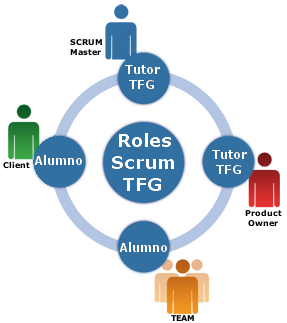
\includegraphics[width=0.5\textwidth]{./figures/ScrumRoles.png}
	\caption{Roles de Scrum para este \acs{TFG}}
	\label{fig:ScrumRoles}
\end{figure}


Aunque la metodología de gestión de proyectos SCRUM esté enfocada para grupos de trabajo, se ajusta de forma extraordinaria a los recursos del \ac{TFG}. Esto es debido a que la función de líder del equipo de desarrollo la puede ejercer el tutor de este trabajo, debido a que posee una gran experiencia a la hora de saber cómo gestionar el desarrollo de un proyecto, mientras que el rol de cliente lo ejerce el alumno, ya que el alumno es quien posee la idea principal del \ac{TFG}. El tutor valora esta idea y propone mejoras en su diseño. Por último, el rol de equipo desarrollador lo puede ejercer solo el alumno ya que es quien implementa el proyecto.

Además, el proceso de funcionamiento de esta metodología se ajusta perfectamente al \ac{TFG} debido a que entre el alumno y el tutor se pueden planificar las tareas que debe desarrollar el alumno, eligiendo cuáles son las más importantes para priorizar en su implementación, de tal forma que se puede planificar la iteración para conseguir el mejor resultado posible con el menor esfuerzo gracias al trabajo en equipo.

En lo referente a la ejecución de la iteración también se ajusta perfectamente a este proyecto, dado que como solo debe hacer el trabajo el alumno se reduce al mínimo el número de objetivos/requisitos en los que el equipo debe trabajar simultáneamente. Adicionalmente, también se van a completar primero los objetivos importantes para el cliente, es decir los que han elegido el alumno y el tutor previamente, de tal forma que si surge algún problema se tiene mucha capacidad de reacción frente a situaciones inesperadas, como por ejemplo si el contexto del proyecto cambia debido a que se prefiere orientar de otra forma. 
 
Acerca de la inspección y adaptación de esta metodología al proyecto, se considera afín. Ya que el alumno y el tutor deciden que día va a ser la próxima reunión para mostrar los resultados. De esta forma se pueden realizar las consideraciones pertinentes acerca de si el trabajo de la iteración necesita alguna adaptación, o bien si la manera de trabajar se puede optimizar mediante las preguntas que realiza el alumno al profesor en las reuniones programadas.
 
\subsection{Herramientas utilizadas para la resolución del proyecto}

A continuación se van a mencionar todas las herramientas utilizadas para el desarrollo del proyecto.

\subsubsection{Software}
\begin{itemize}
\item \ac{IDE} Arduino. Entorno de desarrollo para la programación de las placas Arduino.
\item Bitbucket. Repositorio donde se ha almacenado todo el proyecto.
\item Eclipse. Entorno de desarrollo sobre el que se realiza la programación de los algoritmos que forman el sistema.
\item Fritzing. Programa para la realización de esquemas eléctricos en proyectos con Arduino.
\item Gimp. Programa de manipulación de imágenes sobre el cual se han diseñado y modificado figuras que aparecen en el proyecto.
\item StarUML. Programa para diseñar gráficos \acx{UML} con licencia Open Source.
\item Texmaker. Entorno de desarrollo sobre el que se ha realizado la memoria del proyecto.
\item Vim. Editor de texto utilizado en la programación de algoritmos.
\item Visual Paradigm. Este es un software de modelado \ac{UML} que nos permite analizar, diseñar, codificar, probar y desplegar. Dibuja todo tipo de diagramas \ac{UML}, genera código fuente a partir de dichos diagramas y también posibilita la elaboración de documentos. 
\item Vivado Design Suite. Con el uso de esta herramienta se genera el bitstream necesario para programar la placa \ac{FPGA}
\item Vivado \ac{SDK}. Software necesario para embeber los módulos \acx{IP} desarrollados en Vivado \ac{HLS} en la placa \emph{Zedboard}.
\item Vivado \ac{HLS}. Para poder programar y verificar el funcionamiento de los algoritmos que se desean embeber en la placa.
\item Petalinux. Herramienta necesaria para realizar la compilación cruzada de la aplicación que se desea ejecutar en el procesador \ac{ARM} de la placa.
\item XCTU. Programa necesario para realizar la conexión entre los dos módulos de comunicación \emph{XBee}.
\end{itemize}
\subsubsection{Hardware}
\begin{itemize}
\item Arduino Shield. Imprescindible para poder utilizar los pines de Arduino que no utiliza el controlador Ardumoto.
\item Arduino UNO R3 ATMEGA328. Plataforma computacional con la que se controlan los elementos de prototipado que, en su conjunto, forman el vehículo.
\item Batería recargable \emph{Odec} 9V. Fuente de alimentación del vehículo.
\item Controlador \emph{Sparkfun} Ardumoto. Módulo con el cual se activa y configura el movimiento de los motores.
\item Estación de soldadura JBM AR5800.
\item Imán de neodimio. Utilizado para interactuar con el sensor de efecto Hall.
\item Placa de pruebas para Arduino. Sobre esta placa se establece la instalación de los sensores, leds y resistencias del coche.
\item Placa \emph{Zebdoard} de la marca \emph{Xillinx}. Computador sobre el cual se realizarán los cálculos del sistema.
\item Módulo Xbee de la marca \emph{Digi}. Módulos con los que se realizará la comunicación entre la placa \emph{Zedboard} y Arduino.
\item Osciloscopio y multímetro.
\item Sensor efecto Hall A3144. Utilizado para contar las vueltas que realizan las ruedas del coche.
\end{itemize}